\section{Design}\label{sec:02_design}
% What
This section describes the most important parts of the design of the application. It highlights the database structure and its entities (\Sec{sec:02_design_db}), the purpose and behavior of the EJB`s (\Sec{sec:02_design_beans}), and the behavior of the servlets (\Sec{sec:02_design_web}).


\subsection{Multimodule Project Design}\label{sec:02_design_project}
% What
This application is delivered as a multimodule project. It contains the \textit{DatabaseRoutine}, \textit{WebServices}, and \textit{WebApp} projects, as shown in \Fig{fig:02_design_project_structure}.
% What is what
The \textit{DatabaseRoutine} (introduced in \Sec{sec:02_design_db_routine}) implements the routine to seed the database with test data, \textit{WebServices} contains the business logic, and the \textit{WebApp} project contains the servlets.
% Diagram
\begin{figure}[h]
\centering
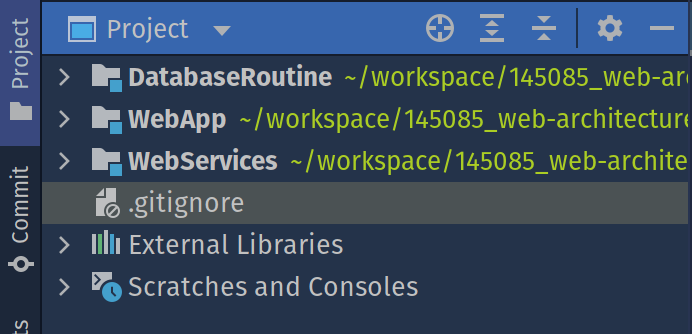
\includegraphics[scale=0.5]{images/02_design/design-project}
\caption{Multimodule project structure}
\label{fig:02_design_project_structure}
\end{figure}


\subsection{Database}\label{sec:02_design_db}
% What
To persist all accommodations, the occupancy of accommodation, and reservations made by the users a database is needed. This application uses an H2 database.

\subsubsection{Structure}\label{sec:02_design_db_structure}
% What Tables
The overall database structure, visualized in \Fig{fig:02_design_db_structure_diagram}, consists of the following three tables:
\begin{itemize}
\item \textit{Accommodation}
\item \textit{Occupancy}
\item \textit{Reservation}
\end{itemize}
% About polymorphism
To enable polymorphism, the \textit{Single Table per Class Hierarchy} strategy is used. This comes with a space inefficiency  disadvantage, however, this application is not intended to save a heavy amount of data. Therefore, it reasonable to use this strategy and have a time efficiency advantage. 

% Diagram
\begin{figure}[h]
\centering
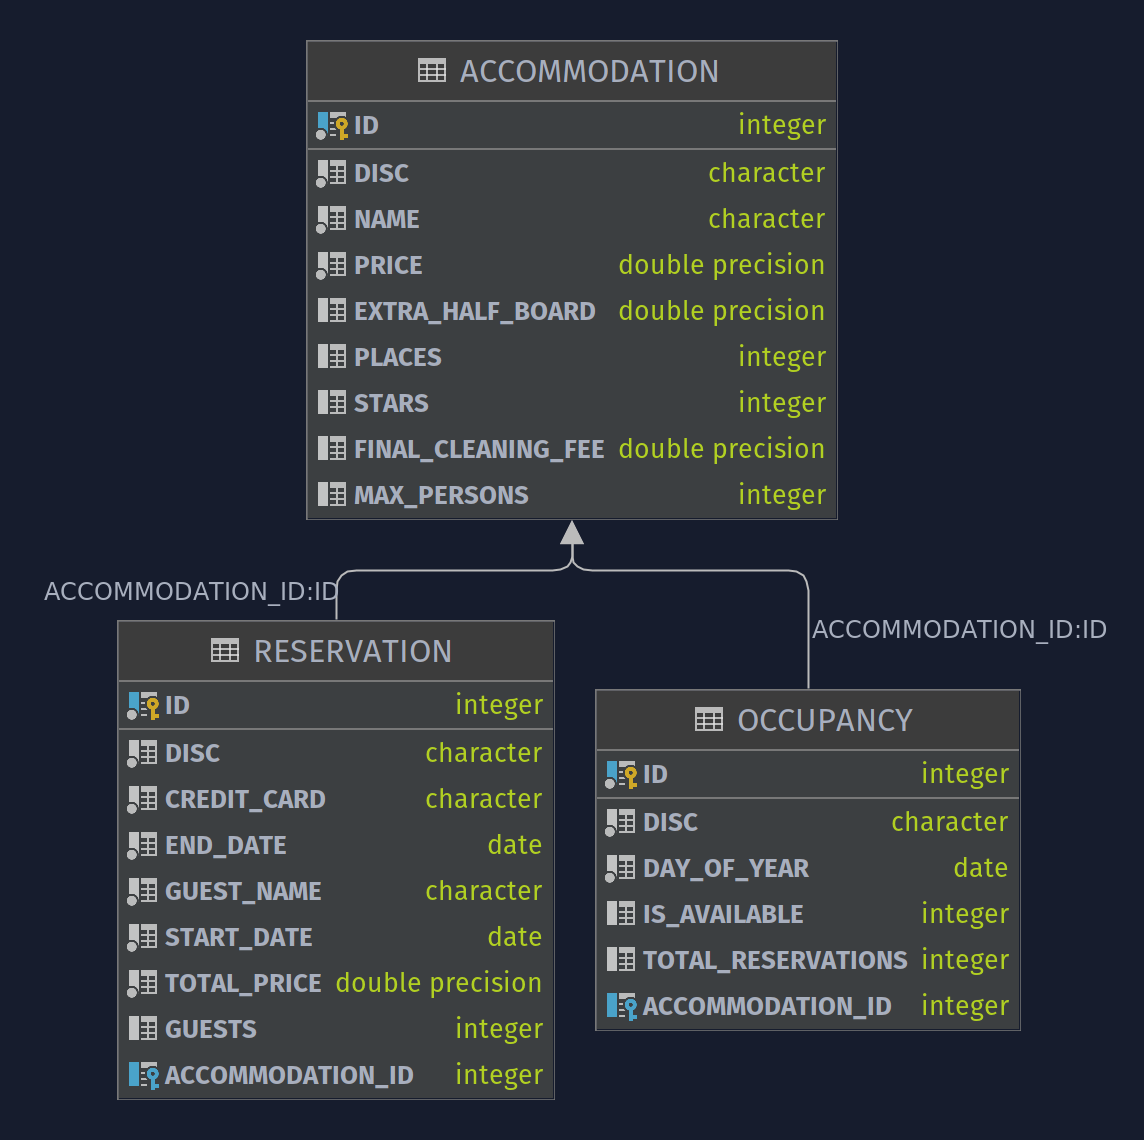
\includegraphics[scale=0.3]{images/02_design/design-database}
\caption{Diagram of the database strcture}
\label{fig:02_design_db_structure_diagram}
\end{figure}

% Explain Tables
\paragraph{Accommodation}
% What
The \textit{Accommodation} table is supposed to save all kinds of accommodation, apartments, and hotels. Both have a name and price. However, an apartment has an additional final cleaning fee, and a number of maximum persons allowed, whereas, a hotel has a rating of stars, a maximum number of places, and a price for an extra half-board.

\paragraph{Occupancy}
% What
The \textit{Occupancy} table saves the occupancy information for an accommodation for a specific date. An occupancy saves a date, and the specific accommodation, where one accommodation can have many occupancies. For an apartment, only a \textit{is available} flag is important, and for a hotel, the number of total reservations for that date is needed.

\paragraph{Reservation}
% What
The \textit{Reservation} table saves all reservations made by all users. It saves the guest's name, the guest's credit card number, the start and end date, and the total price for the reservation. Additionally, for a hotel reservation, it is needed to save the number of guests as well. Accommodations and reservations are in a one-to-many relationship, where one accommodation can have many reservations.

\subsubsection{Entities}\label{sec:02_design_db_entities}
% What
To use the database in code, the application uses the Hibernate Object Relationship Mapping (ORM), in conjunction with the Java Persistence API (JPA). \Fig{fig:02_design_db_entities_uml} visualizes the UML diagram of the entities used to map the database structure (introduced in \Sec{sec:02_design_db_structure}).
% UML
\begin{figure}[h]
\centering
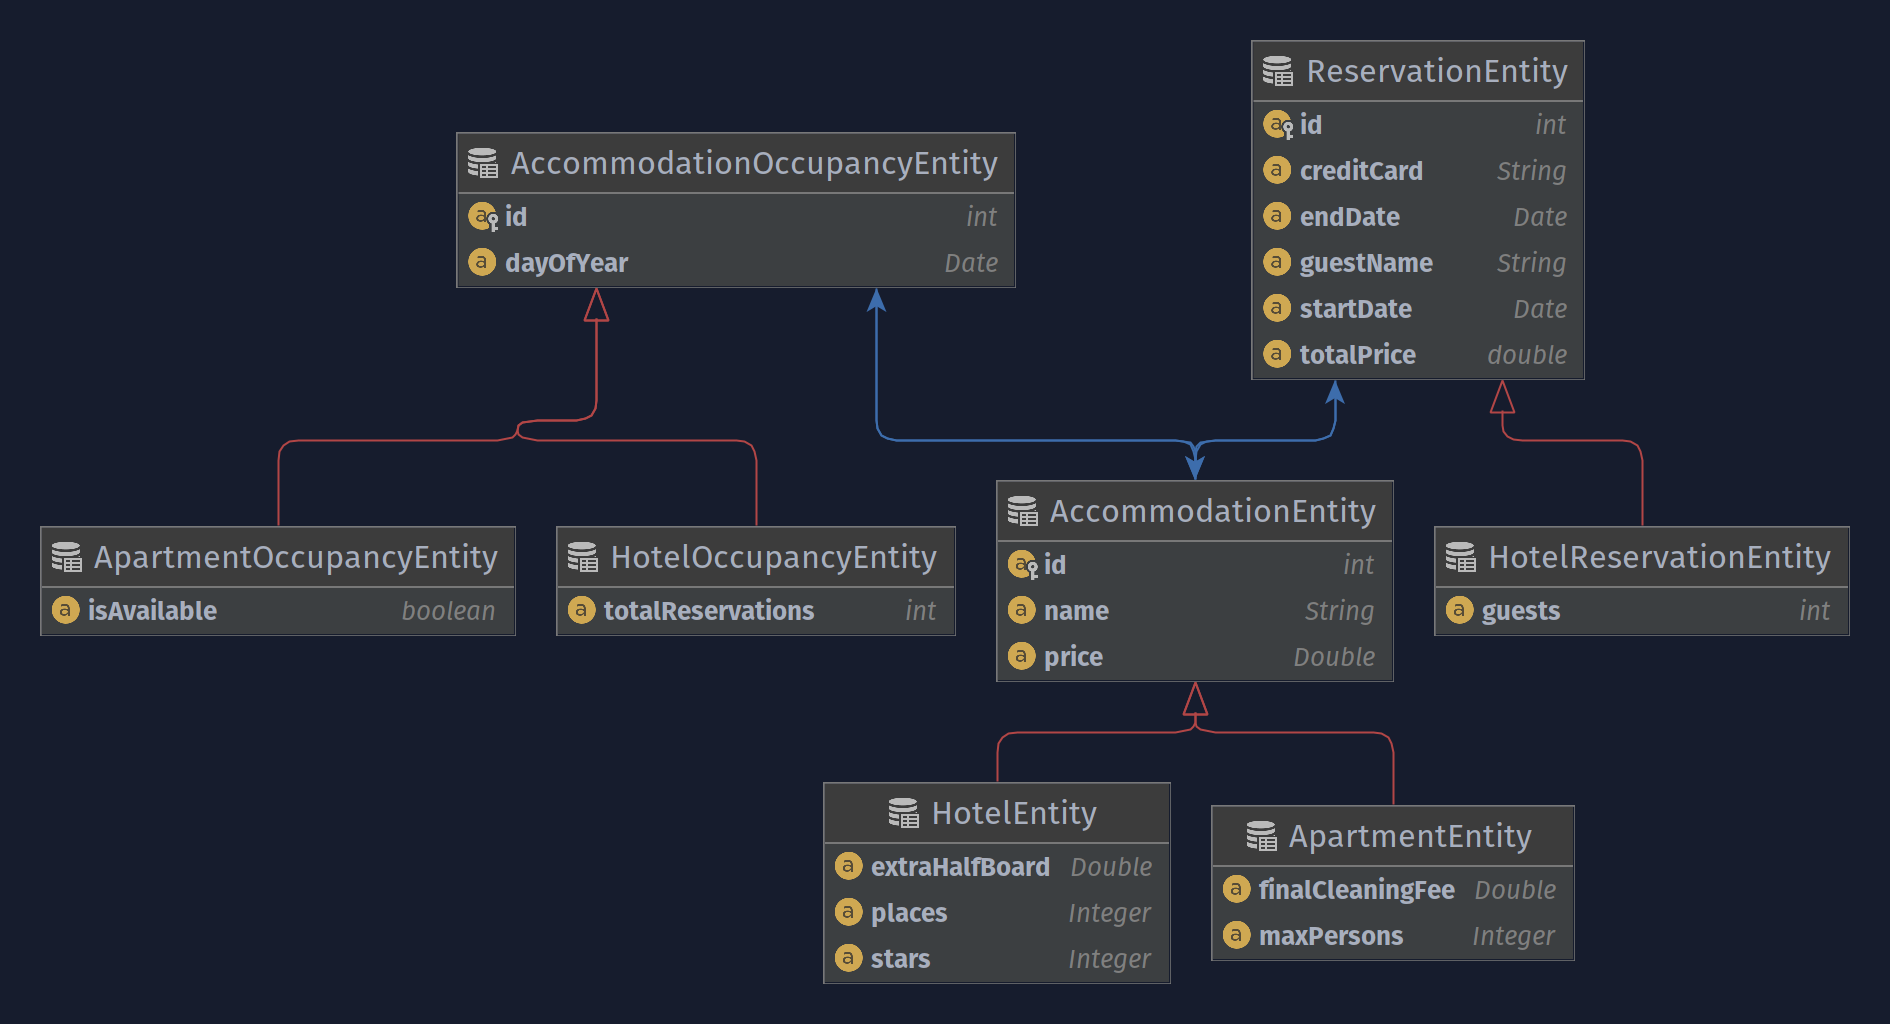
\includegraphics[scale=0.22]{images/02_design/design-entities}
\caption{Database entities UML diagram}
\label{fig:02_design_db_entities_uml}
\end{figure}
% Overall
Overall, the following entities are used in the implementation:
\begin{itemize}
\item \textit{AccommodationEntity}
\begin{itemize}
\item \textit{ApartmentEntity}
\item \textit{HotelEntity}
\end{itemize}

\item \textit{AccommodationOccupancyEntity}
\begin{itemize}
\item \textit{ApartmentOccupancyEntity}
\item \textit{HotelOccupancyEntity}
\end{itemize}

\item \textit{ReservationEntity}
\begin{itemize}
\item \textit{HotelReservationEntity}
\end{itemize}
\end{itemize}


% Accommodatins
\paragraph{AccommodationEntity}
% What 
The \textit{AccommodationEntity} represents the \textit{Accommodation} table (introduced in \Sec{sec:02_design_db_structure}). It is an abstract class and has two child classes, the \textit{ApartmentEntity}, and the \textit{HotelEntity}, which represent an apartment and a Hotel respectively.

% Occupancies
\paragraph{AccommodationOccupancyEntity}
% What
The \textit{AccommodationOccupancyEntity} represents the \textit{Occupancy} table. It is an abstract class as well and has two child classes, the \textit{ApartmentOccupancyEntity}, and the \textit{HotelOccupancyEntity}. Both child classes, save the occupancy information of either an apartment or a hotel.


% Reservations
\paragraph{ReservationEntity}
% What 
The \textit{ReservationEntity} represents the \textit{Reservation} table. If a reservation is made for an apartment, it saves a plain \textit{ReservationEntity} to the database. Otherwise, if a reservation has been made for a hotel, a \textit{HotelReservationEntity} is saved to the database.

\subsubsection{Database Routine}\label{sec:02_design_db_routine}
% Intro
To seed the database with test data, the \textit{DatabaseRoutine} project has been implemented.
% No EJB
This project is not implemented as an EJB, instead, it will run as a standalone Java application.
% Technology
To utilize the database, this project uses Hibernate and JPA.


% =====================
% =====================
\newpage
\subsection{Enterprise Java Beans}\label{sec:02_design_beans}
% Business logic
The business logic of this application is implemented using three EJB`s:
\begin{itemize}
\item \textit{LocalDatabaseBean}
\item \textit{AccommodationService}
\item \textit{ReservationService}
\end{itemize}
% One Project
All services are part of a single Maven project called \textit{WebServices}.

% What
Each part (service) is an independent EJB. The client can look up the EJB given an address and invoke methods on it. Only the \textit{AccommodationService} and the \textit{ReservationService} are available for the client. Both utilize the \textit{Facade} pattern, to encapsulate the complexity to work with entities (introduced in \Sec{sec:02_design_db_entities}) directly and are stateless Beans, because this project does not require any authentication, and therefore keeping state is not required. The \textit{DatabaseService} is implemented as a local bean because it is not intended for the user to interact with the database directly.


\subsubsection{LocalDatabaseBean}\label{sec:02_design_beans_local}
% What
The \textit{LocalDatabaseBean} is used to interact with the H2 database. It initiates the \textit{EntityManager}, given by JPA, to establish a connection to a JTA data source. Other services can use the \textit{DatabaseService} to send queries and receive results from the database.

% How
As mentioned before, the \textit{DatabaseService} is implemented as a \texttt{LocalBean}. Other EJB`s can interact with the \textit{DatabaseService} using the code-injection pattern, which is shown in \Lst{lst:02_design_ejb_db_cinjection}.
% The implementation
\begin{lstlisting}[label=lst:02_design_ejb_db_cinjection, caption=Usage of the \textit{LocalDatabaseBean} using code-injection, language=java]
@Stateless
@Remote(ReservationService.class)
public class ReservationBean implements ReservationService  {
    @EJB()
    private LocalDatabaseBean databaseBean;
    ...
}
\end{lstlisting}


\subsubsection{AccommodationService}\label{sec:02_design_beans_acc}
% What
The \textit{AccommodationService} is used by the client to interact with the \textit{AccommdationEntity} and its child classes \textit{ApartmentEntity}, and \textit{HotelEntity} (introduced in \Sec{sec:02_design_db_entities}). It uses the \textit{LocalDatabaseBean} to send queries to the H2 database.

% Getting available accommodations
Except for receiving accommodations based on specific properties, the most interesting part about \textit{AccommodationService} is how it receives available accommodations in a specific date range, given the number of guests.
% How
The idea is, that the number of occurrences of an accommodation that is available in the specific date range, has to be equal to the number of days of the given date range.
% SQL
\begin{lstlisting}[label=lst:02_design_ejb_accommodation_sql, caption=Example of a HQL query to receive all available accommodations, language=sql]
SELECT a.accommodation
FROM AccommodationOccupancyEntity a
WHERE (
  ((a.isAvailable IS TRUE AND a.accommodation.maxPersons >= 2) 
  OR 
  ((a.accommodation.places - a.totalReservations) >= 2))
)
AND a.dayOfYear BETWEEN '2022-02-01' AND '2022-02-09'
GROUP BY a.accommodation.id
HAVING COUNT(*) = 9 
\end{lstlisting}
% Describe
\Lst{lst:02_design_ejb_accommodation_sql} shows an example HQL (Hibernate Query Language) query, to get all available accommodations between 1. February 2022 and 10. February 2022 for 2 guests.
As described before, the \texttt{AccommodationOccupancyEntity} saves the occupancies of each accommodation for specific dates. Therefore, it is necessary to check for apartments if it is available, and has enough places for the number of guests. For hotels, it is necessary to check if the existing number of reservations minus the available places of that hotel is lower or equal to the number of guests.
These constraints are checked for the range between the start date (1. February 2022) and the end date minus one day (9. February 2022). It is necessary to subtract one day, because the guests will not stay for the last day, and therefore the availability information for this day is unrelated.
After that, it is important, that the count of numbers of the accommodation, in that specific date range, is equal to the number of days between the start and end date.


\subsubsection{ReservationService}\label{sec:02_design_beans_reservation}
% Describe
To read from and write to the reservation table of the database, the \textit{ReservationService} is used. It allows to persist new reservations to the database and to get all reservations for a specific customer name.

% Adding new reservations
When adding a new reservation to the database, the \textit{ReservationService} is also responsible to update the occupancies (mentioned in \Sec{sec:02_design_db_structure}) of the selected accommodation. Then, it is necessary to add the number of guests, of the new reservation, to each entry of the accommodation occupancy.

% Calculating the price
Additionally, the \textit{ReservationService} provides an interface to calculate the price of a reservation for either a Hotel or an Apartment.

\newpage
\subsubsection{Build Process}\label{sec:02_design_beans_build}
% Jar
The project is built using the \texttt{maven-ejb-plugin} maven plugin to create an EJB JAR artifact.
% How
Then, the artifact can be built using the \texttt{mvn clean build} command.

% Settings
\Lst{lst:02_design_ejb_buildprocess_pluginconfig} shows the configuration of the \texttt{maven-ejb-plugin} plugin.
% Config
\begin{lstlisting}[label=lst:02_design_ejb_buildprocess_pluginconfig, caption=\texttt{maven-ejb-plugin} plugin configuration, language=xml]
<packaging>ejb</packaging>
...
<build>
  <finalName>${artifactId}.${version}</finalName>
  <plugins>
    <plugin>
      <groupId>org.apache.maven.plugins</groupId>
      <artifactId>maven-ejb-plugin</artifactId>
      <version>3.1.0</version>
    </plugin>
  </plugins>
</build>
\end{lstlisting}



% =====================
% =====================
\subsection{Web Application}\label{sec:02_design_web}
% What
The \textit{WebApp} project implements the presentation layer of the application. Additionally, it constructs the EJB`s (introduced in \Sec{sec:02_design_beans}) for the business logic and presents the results to the client.
 
% What parts
It consists of the following servlets:
\begin{itemize}
\item \textit{AccommodationSearchServlet}
\item \textit{AccommodationResultServlet}
\item \textit{ReservationSummaryServlet}
\item \textit{ReservationConfirmServlet}
\item \textit{ReservationListServlet}
\end{itemize}

\subsubsection{EJB Patterns}\label{sec:02_design_web_patterns}
% Which patterns
To utilize the EJB`s (introduced in \Sec{sec:02_design_beans}) on the client side the \textit{WebApp} project uses the \textit{Singleton}, \textit{Simple Factory}, and \textit{Business Delegate} patterns.

% What classes
The helper classes, which uses these patterns are:
\begin{itemize}
\item \textit{ServiceLocator}
\item \textit{ServiceFactory}
\item \textit{AccommodationServiceDelegate}
\item \textit{ReservationServiceDelegate}
\end{itemize}

\paragraph{ServiceLocator}
% What pattern
The \textit{ServiceLocator} is responsible for lookup for a remote Bean given an address. After that, it can be used recreated and used on the client. Internally, it uses the \textit{Singleton} pattern. \Lst{lst:02_design_web_pattern_servicelocator} shows an example of how the AccommodationServe can be constructed using the \textit{ServiceLocator}.
% Example
\begin{lstlisting}[label=lst:02_design_web_pattern_servicelocator, caption=Example usage of the \textit{ServiceLocator}, language=java]
String serviceAddress = getAccommodationbeanAddress();
AccommodationService service = ServiceLocator.getInstance().getService(serviceAddress);
service.getAccommodations();
\end{lstlisting}

\paragraph{ServiceFactory}
% What
The usage of the \textit{ServiceLocator} still requires some boilerplate code, each time an EJB Bean needs to be constructed, for example, the generator of the Bean address. To simplify this process, the \textit{ServiceFactory} uses the \textit{Simple Factory} pattern to construct EJB Beans based on its name. \Lst{lst:02_design_web_pattern_servicefactory} shows an example of how to use the \textit{ServiceFactory} to construct the \textit{AccommodationService}.
\begin{lstlisting}[label=lst:02_design_web_pattern_servicefactory, caption=Example usage of the \textit{ServiceFactory}, language=java]
AccommodationService service = ServiceFactory.initializeService(
  "AccommodationService",
  AccommodationService.class.getName()
);
\end{lstlisting}

\paragraph{Business Delegates}
% Why
The \textit{AccommodationDelegate} and \textit{ReservationDelegate} both use the \textit{Business Delegate} pattern, to abstract the usage of the \textit{AccommodationService} and \textit{ReservationService} respectively. The servlets controller (previously mentioned in \Sec{sec:02_design_web}) uses these \textit{Business Delegates}, instead of constructing and invoking methods on the remote Beans directly. To construct the Beans, the \textit{Business Delegates} use the \textit{ServiceFactory} internally.

\newpage
\subsubsection{AccommodationSearchServlet}\label{sec:02_design_web_search}
% What
The \textit{AccommodationSearchServlet} is the start page of the \textit{WebApp} and provides the search to search for available accommodations, as shown in \Fig{fig:02_design_web_search_page}.

% Form
The user can set the start, and end date of the duration, as well as the number of persons who intend to be in the accommodation during that time.
% Request
After submitting the form, the servlet sends a GET request with the given data to the \textit{AccommodationResultServlet}.
% Figure
\begin{figure}[h]
\centering
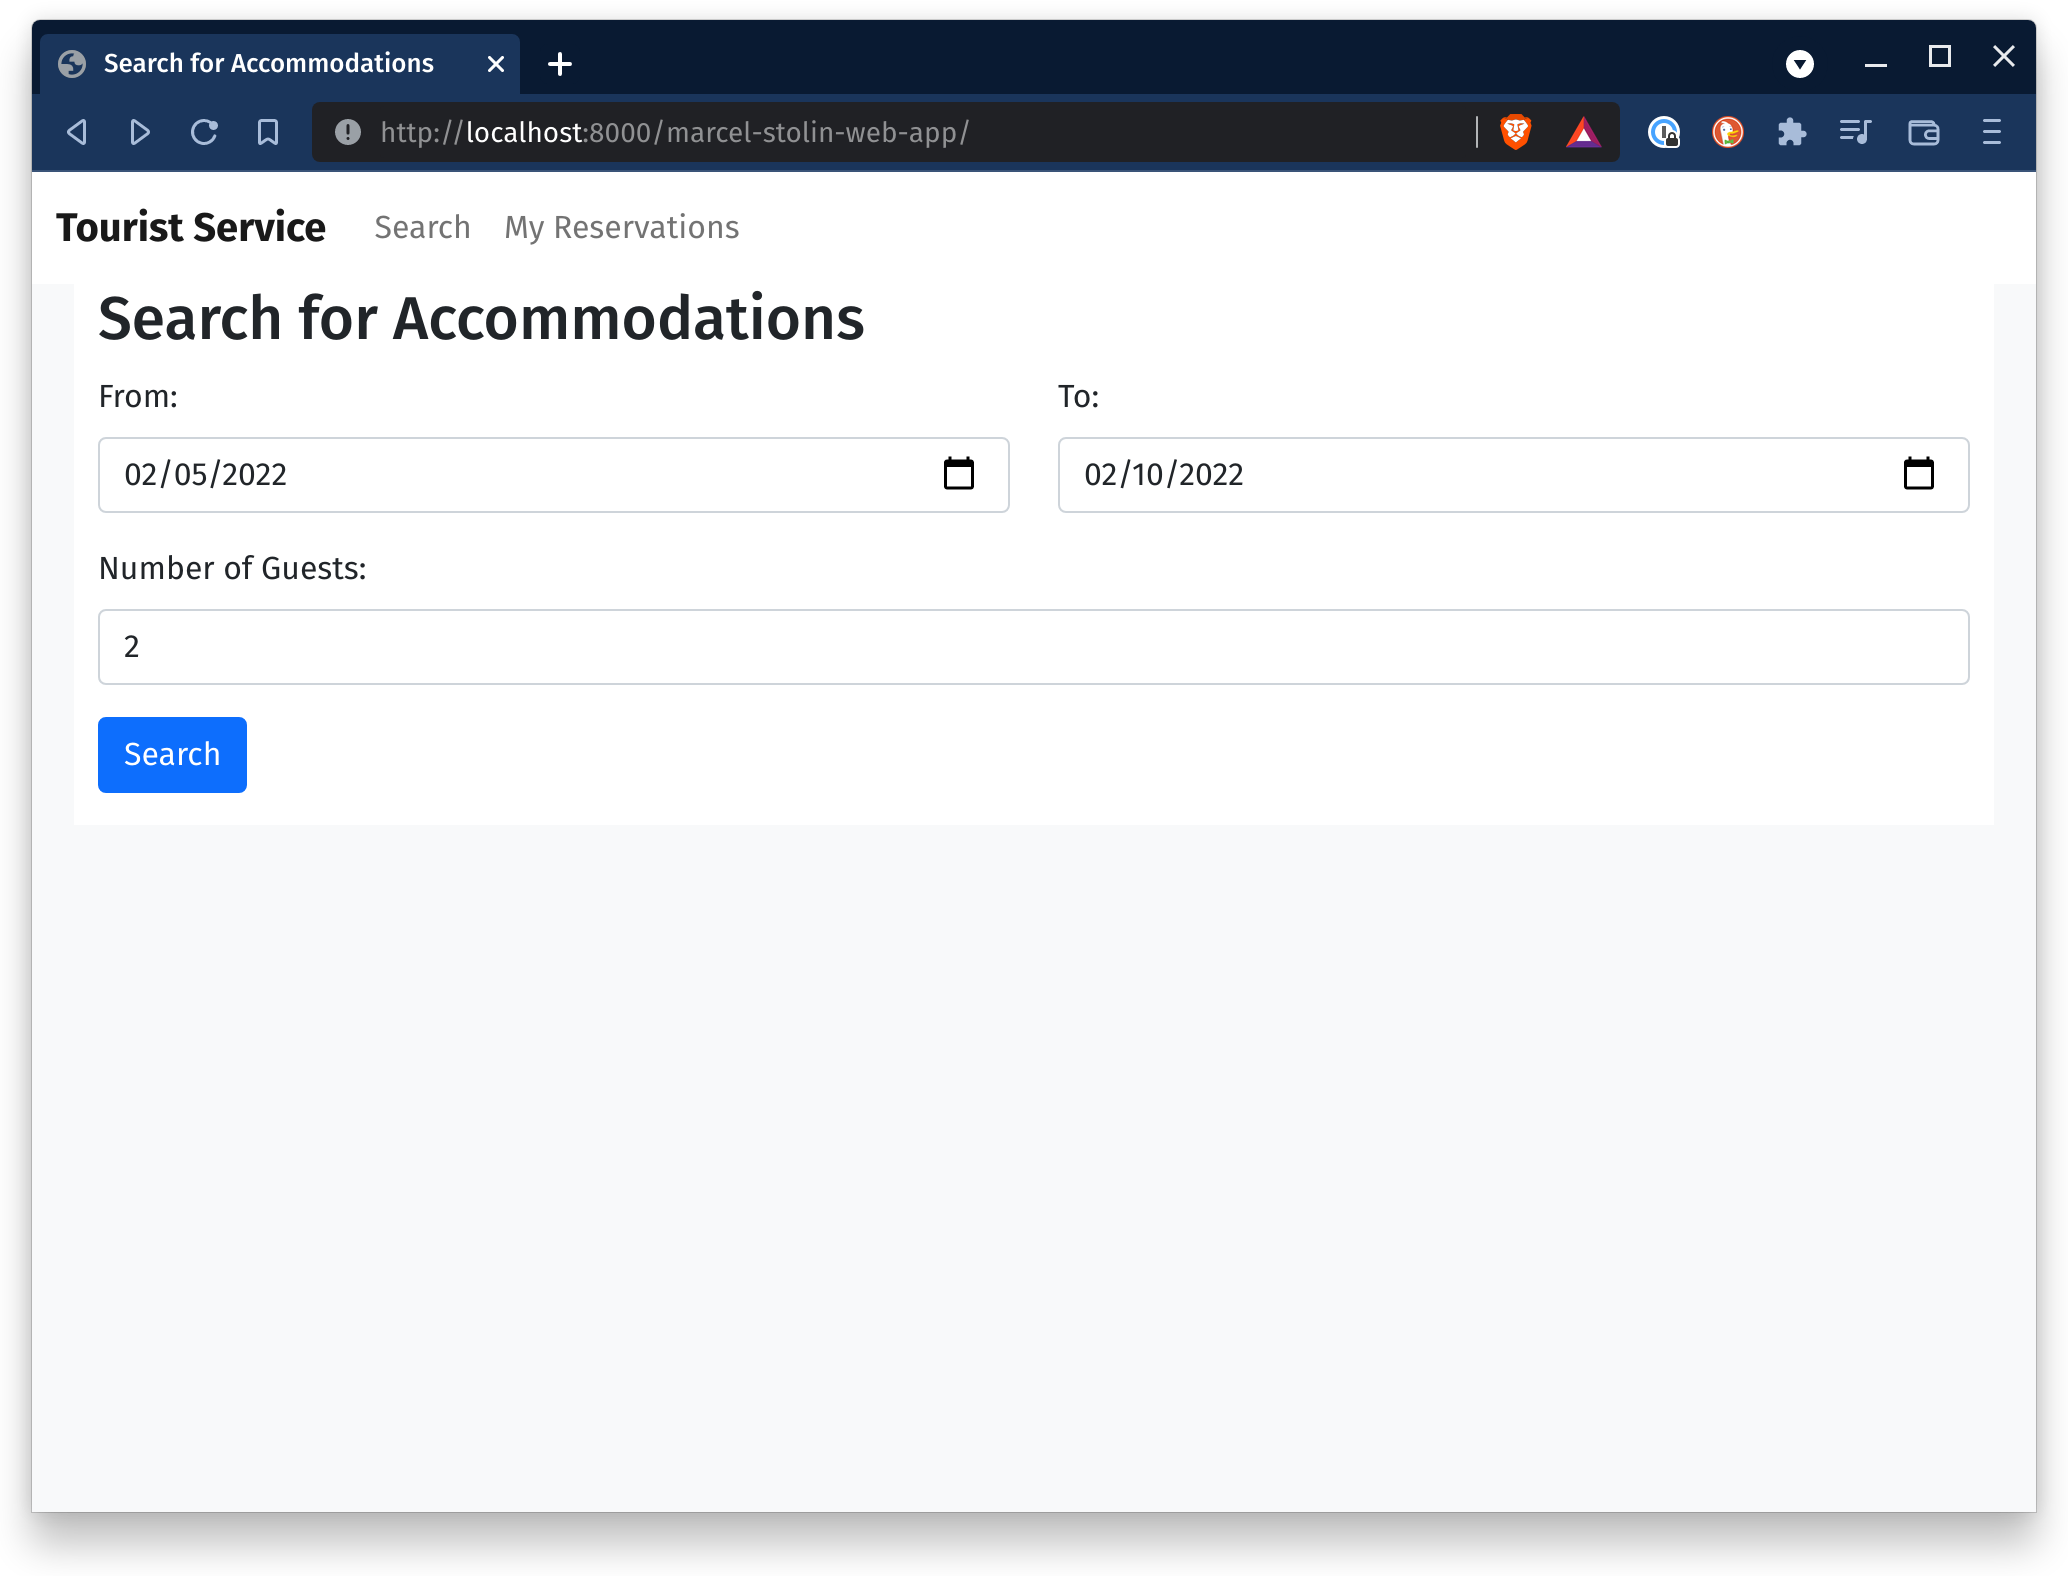
\includegraphics[scale=0.14]{images/02_design/web-app-search}
\caption{UI of the \textit{AccommodationSearchServlet}}
\label{fig:02_design_web_search_page}
\end{figure}

\subsubsection{AccommodationResultServlet}\label{sec:02_design_web_results}
% What
After submitting the search form, the \textit{AccommodationResultServlet} is responsible to present the results.
% No results
If no accommodations are available for the given specifications, a message is shown.
% We have results
Otherwise, a grid of all available results, order by the daily price, is presented to the user, as shown in \Fig{fig:02_design_web_results_page}. There, the user can click on the \textit{Book} button to open the \textit{ReservationSummaryServlet}. If the accommodation is a \textit{Hotel} entity, two buttons are shown, one for the total price without half-board, and on including half-board.
% Figure
\begin{figure}[h]
\centering
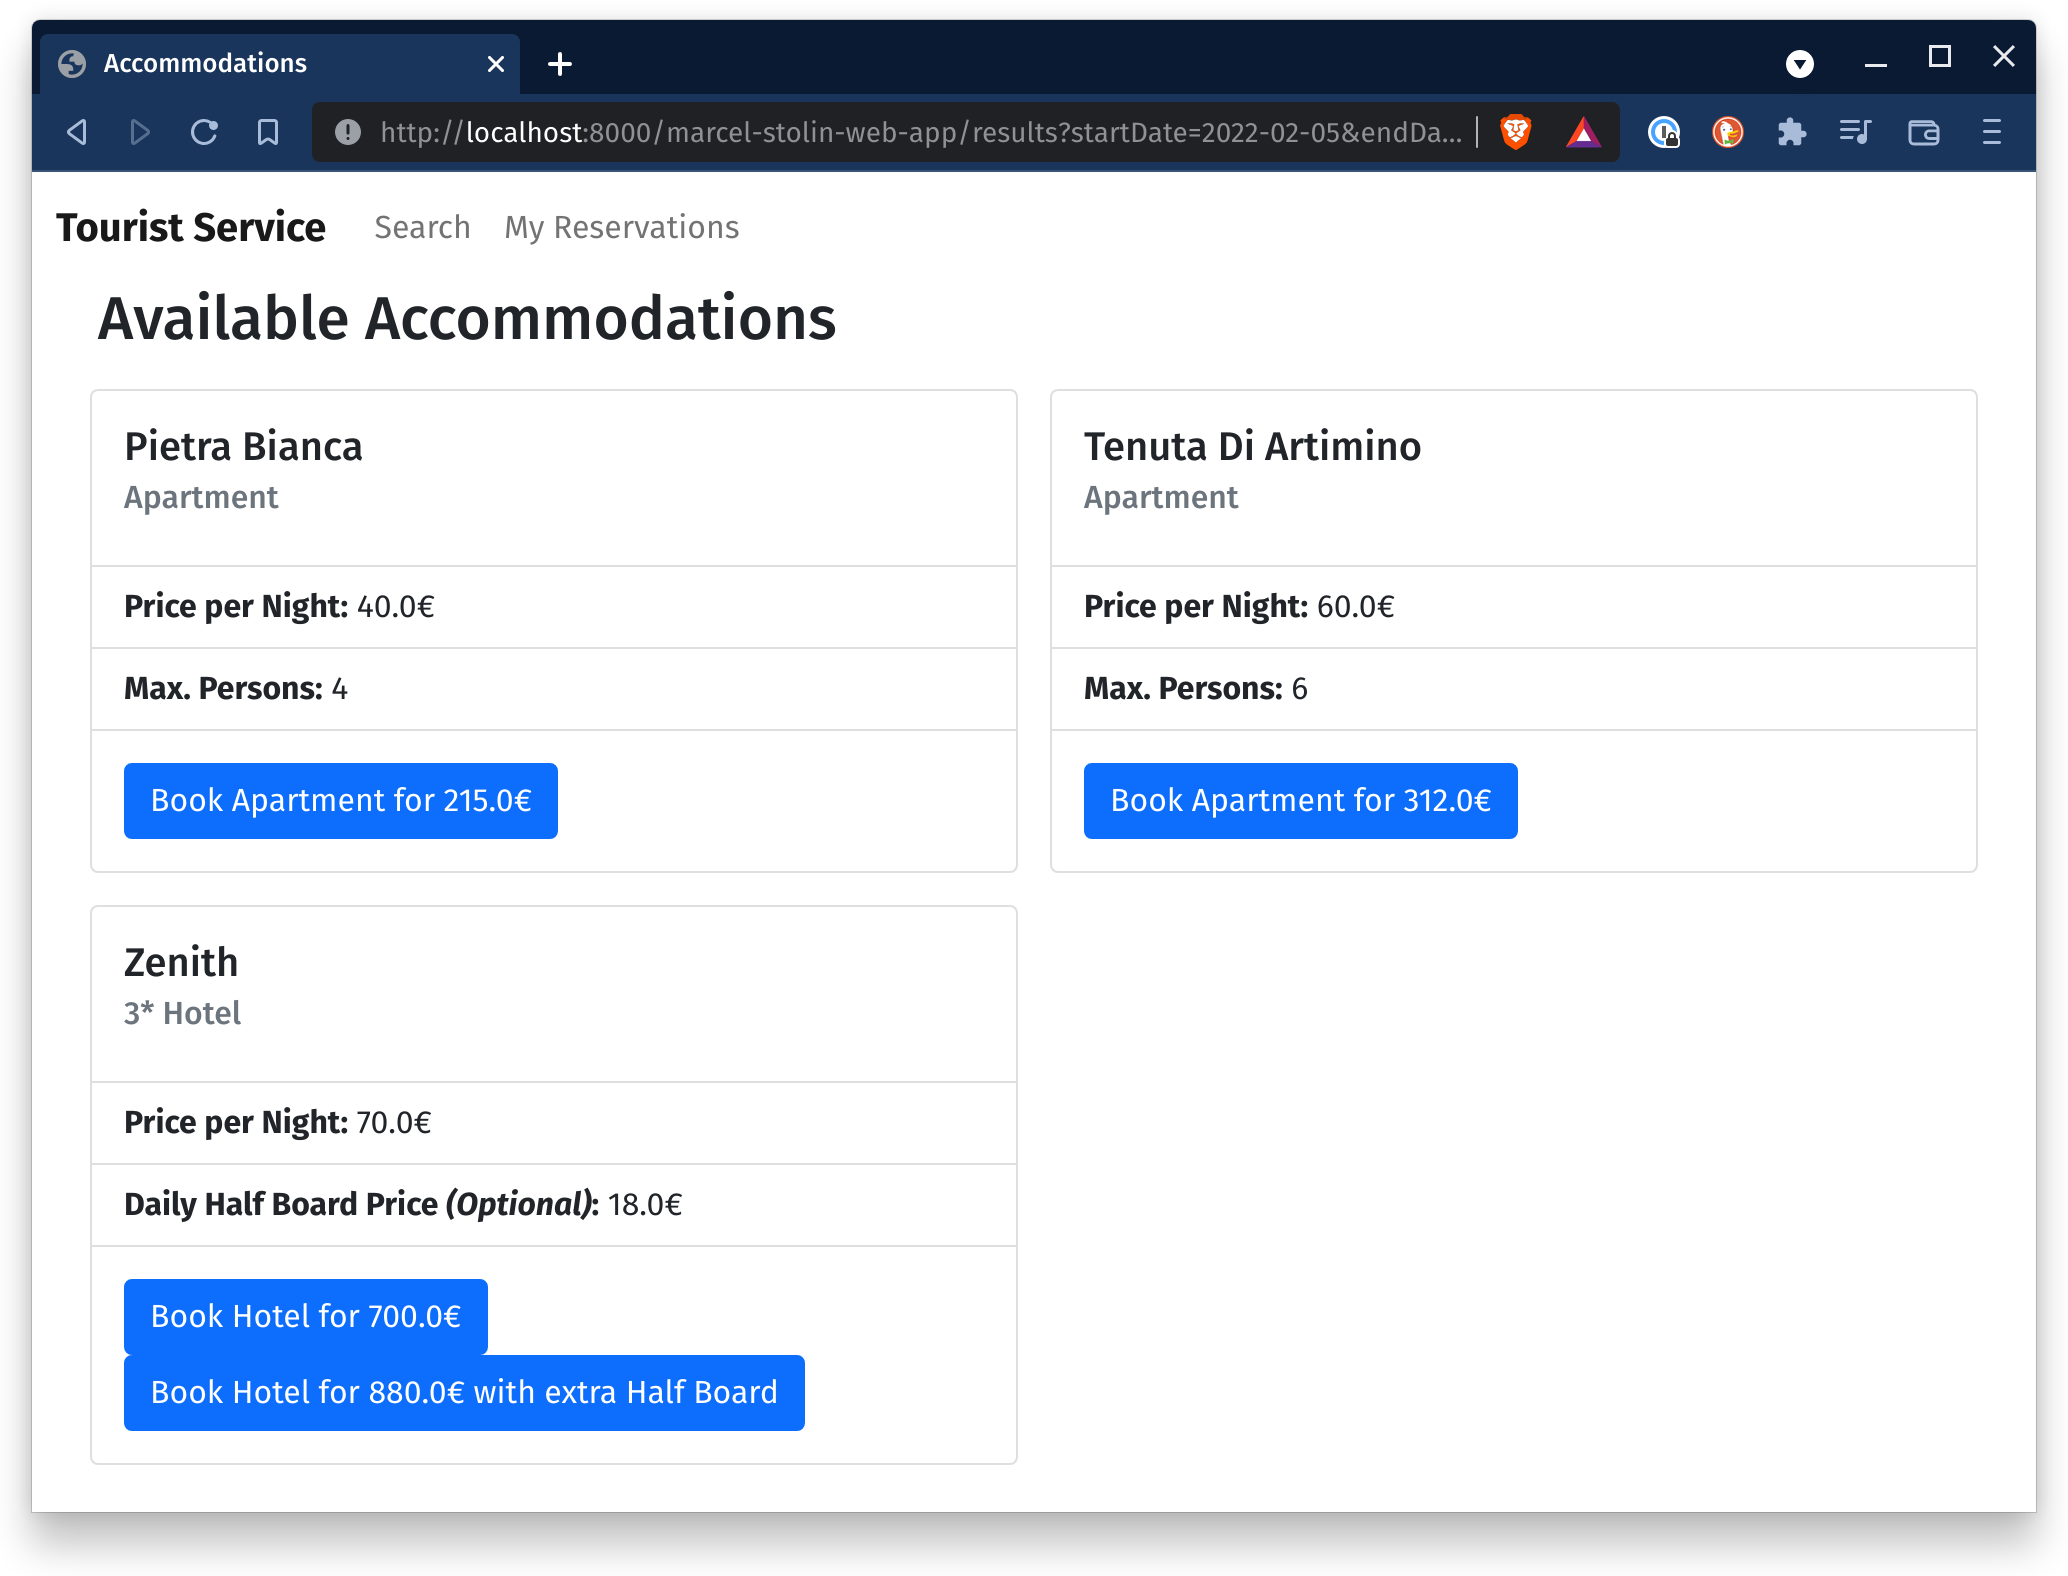
\includegraphics[scale=0.14]{images/02_design/web-app-results}
\caption{UI of the \textit{AccommodationResultServlet}}
\label{fig:02_design_web_results_page}
\end{figure}

\newpage
\subsubsection{ReservationSummaryServlet}\label{sec:02_design_web_reservationsummary}
% What
In the \textit{ReservationSummaryServlet} the user can see a summary after selecting an accommodation at the \textit{AccommodationResultServlet}, as shown in \Fig{fig:02_design_web_reservationsummary_page}.
% Submitting reservation
Additionally, at this point, the user has the opportunity to confirm the reservation by clicking the \textit{Confirm} button or canceling the reservation by clicking the \textit{Cancel} button.
% POST
If the user decides to confirm the reservation, the user has to provide a first name, last name, and a credit card number. Then, a POST request is sent to the \textit{ReservationConfirmServlet}.

% Figure
\begin{figure}[h]
\centering
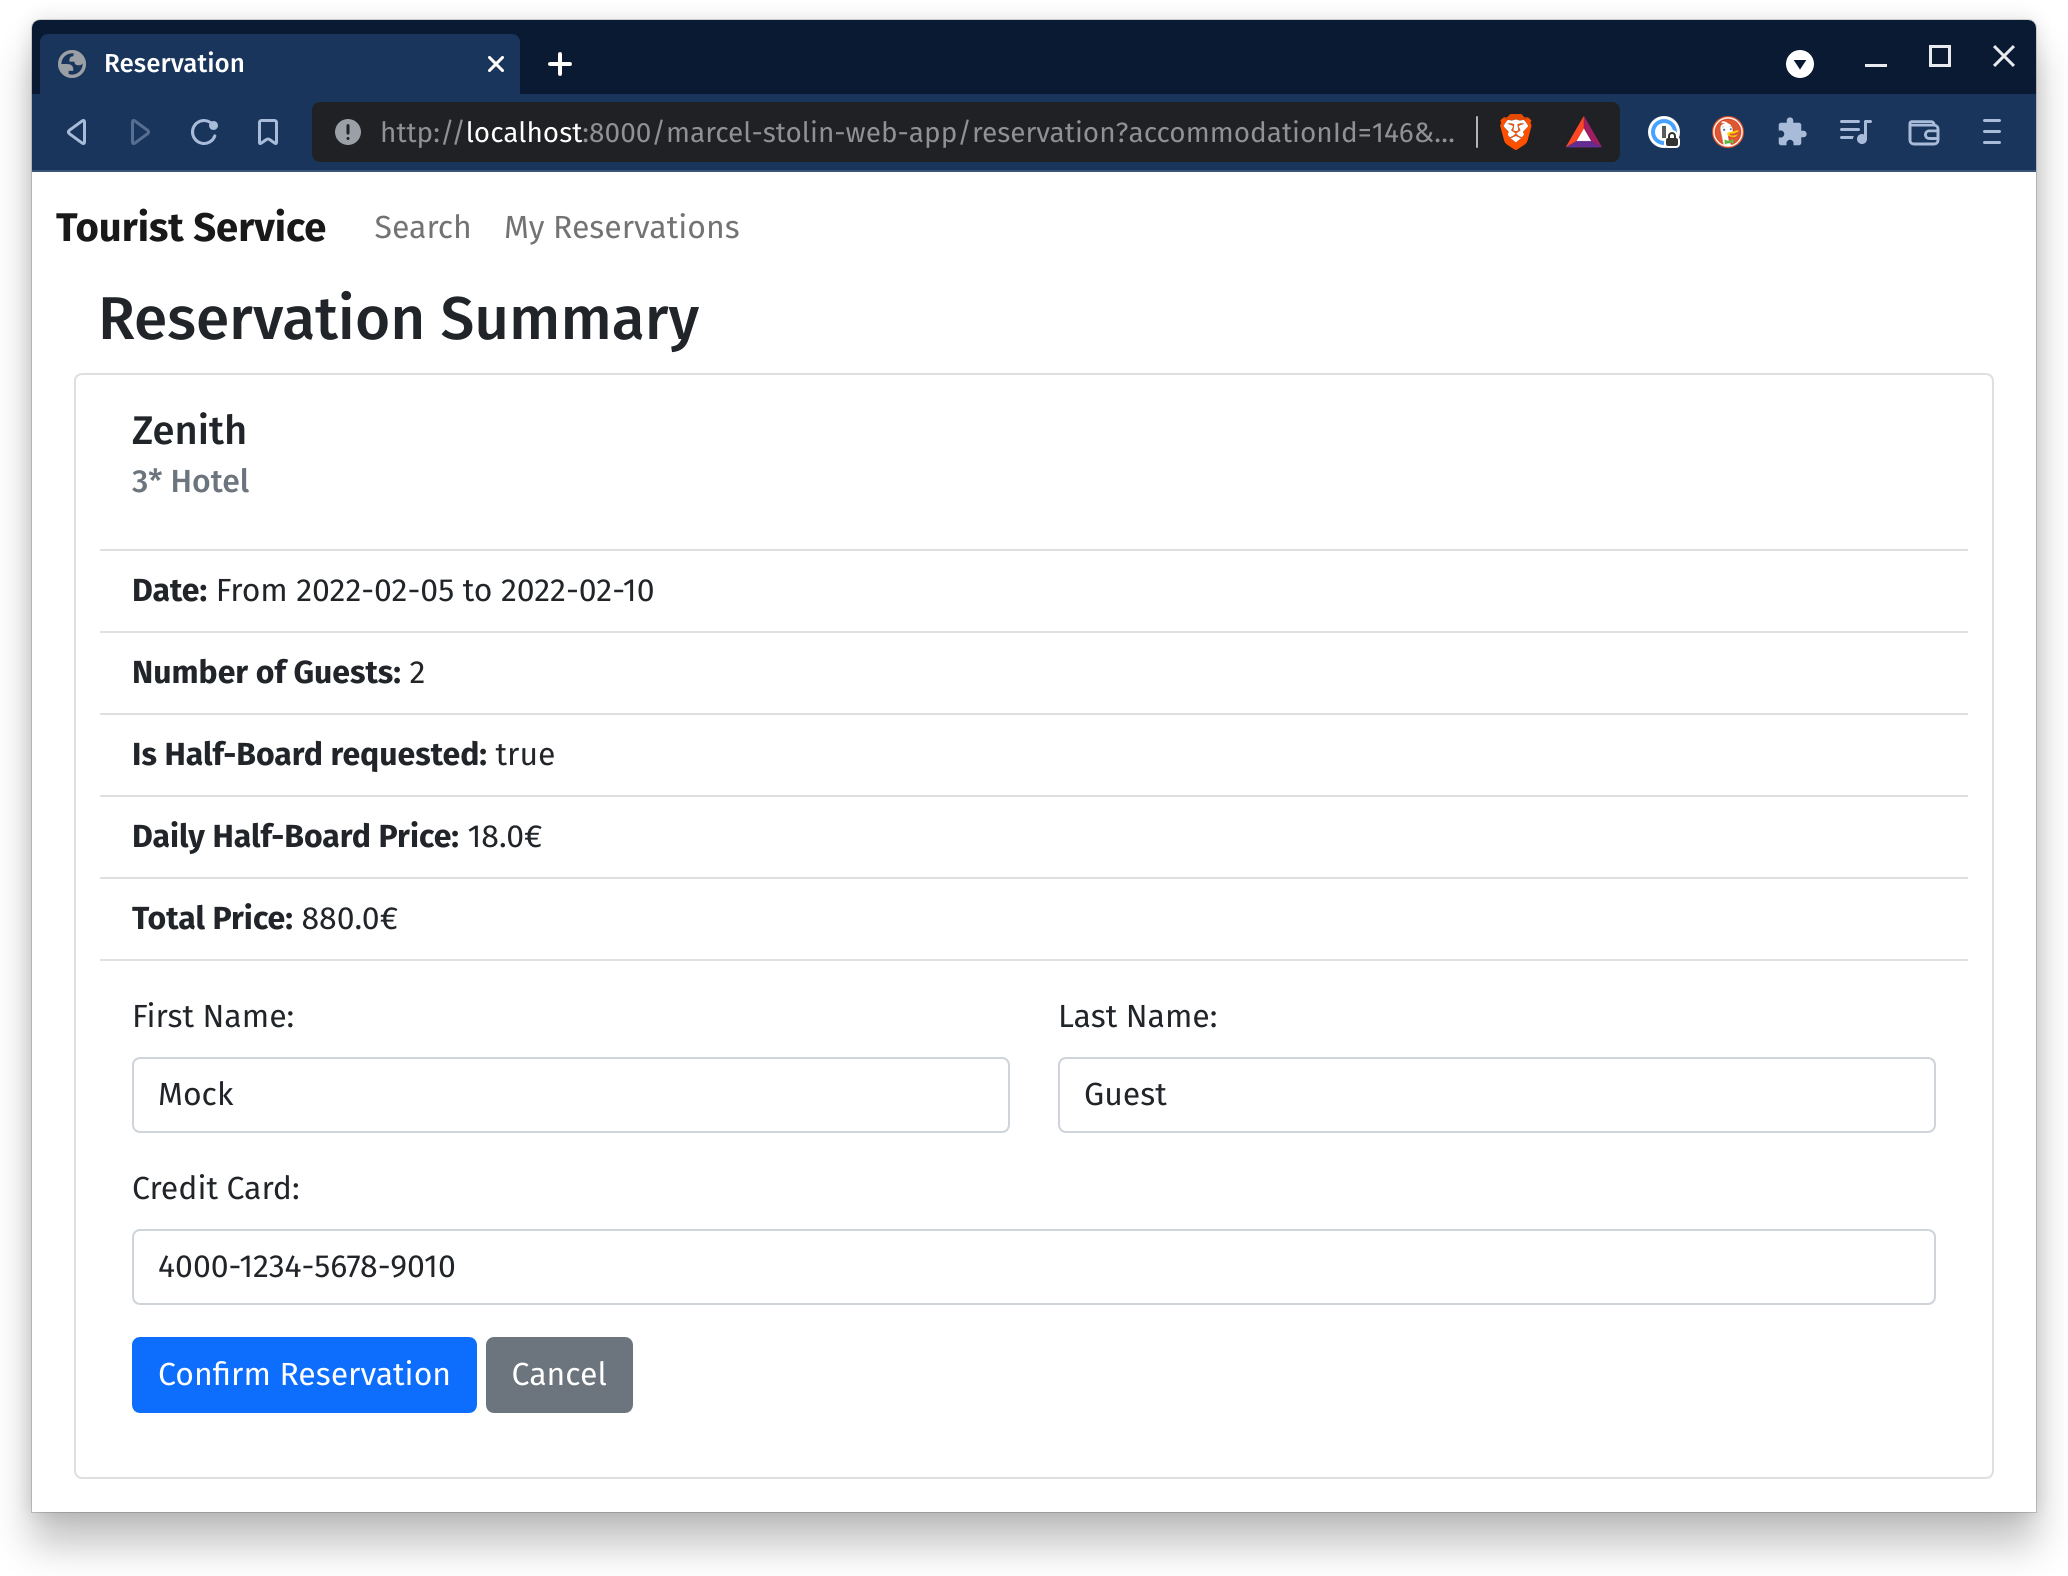
\includegraphics[scale=0.14]{images/02_design/web-app-reservation-summary}
\caption{UI of the \textit{ReservationSummaryServlet}}
\label{fig:02_design_web_reservationsummary_page}
\end{figure}

\newpage
\subsubsection{ReservationConfirmServlet}\label{sec:02_design_web_reservationconfirm}
% What
The \textit{ReservationConfirmServlet} is responsible to save a reservation, and showing the user a success message, as illustrated in \Fig{fig:02_design_web_reservationconfirm_page}.

% Figure
\begin{figure}[h]
\centering
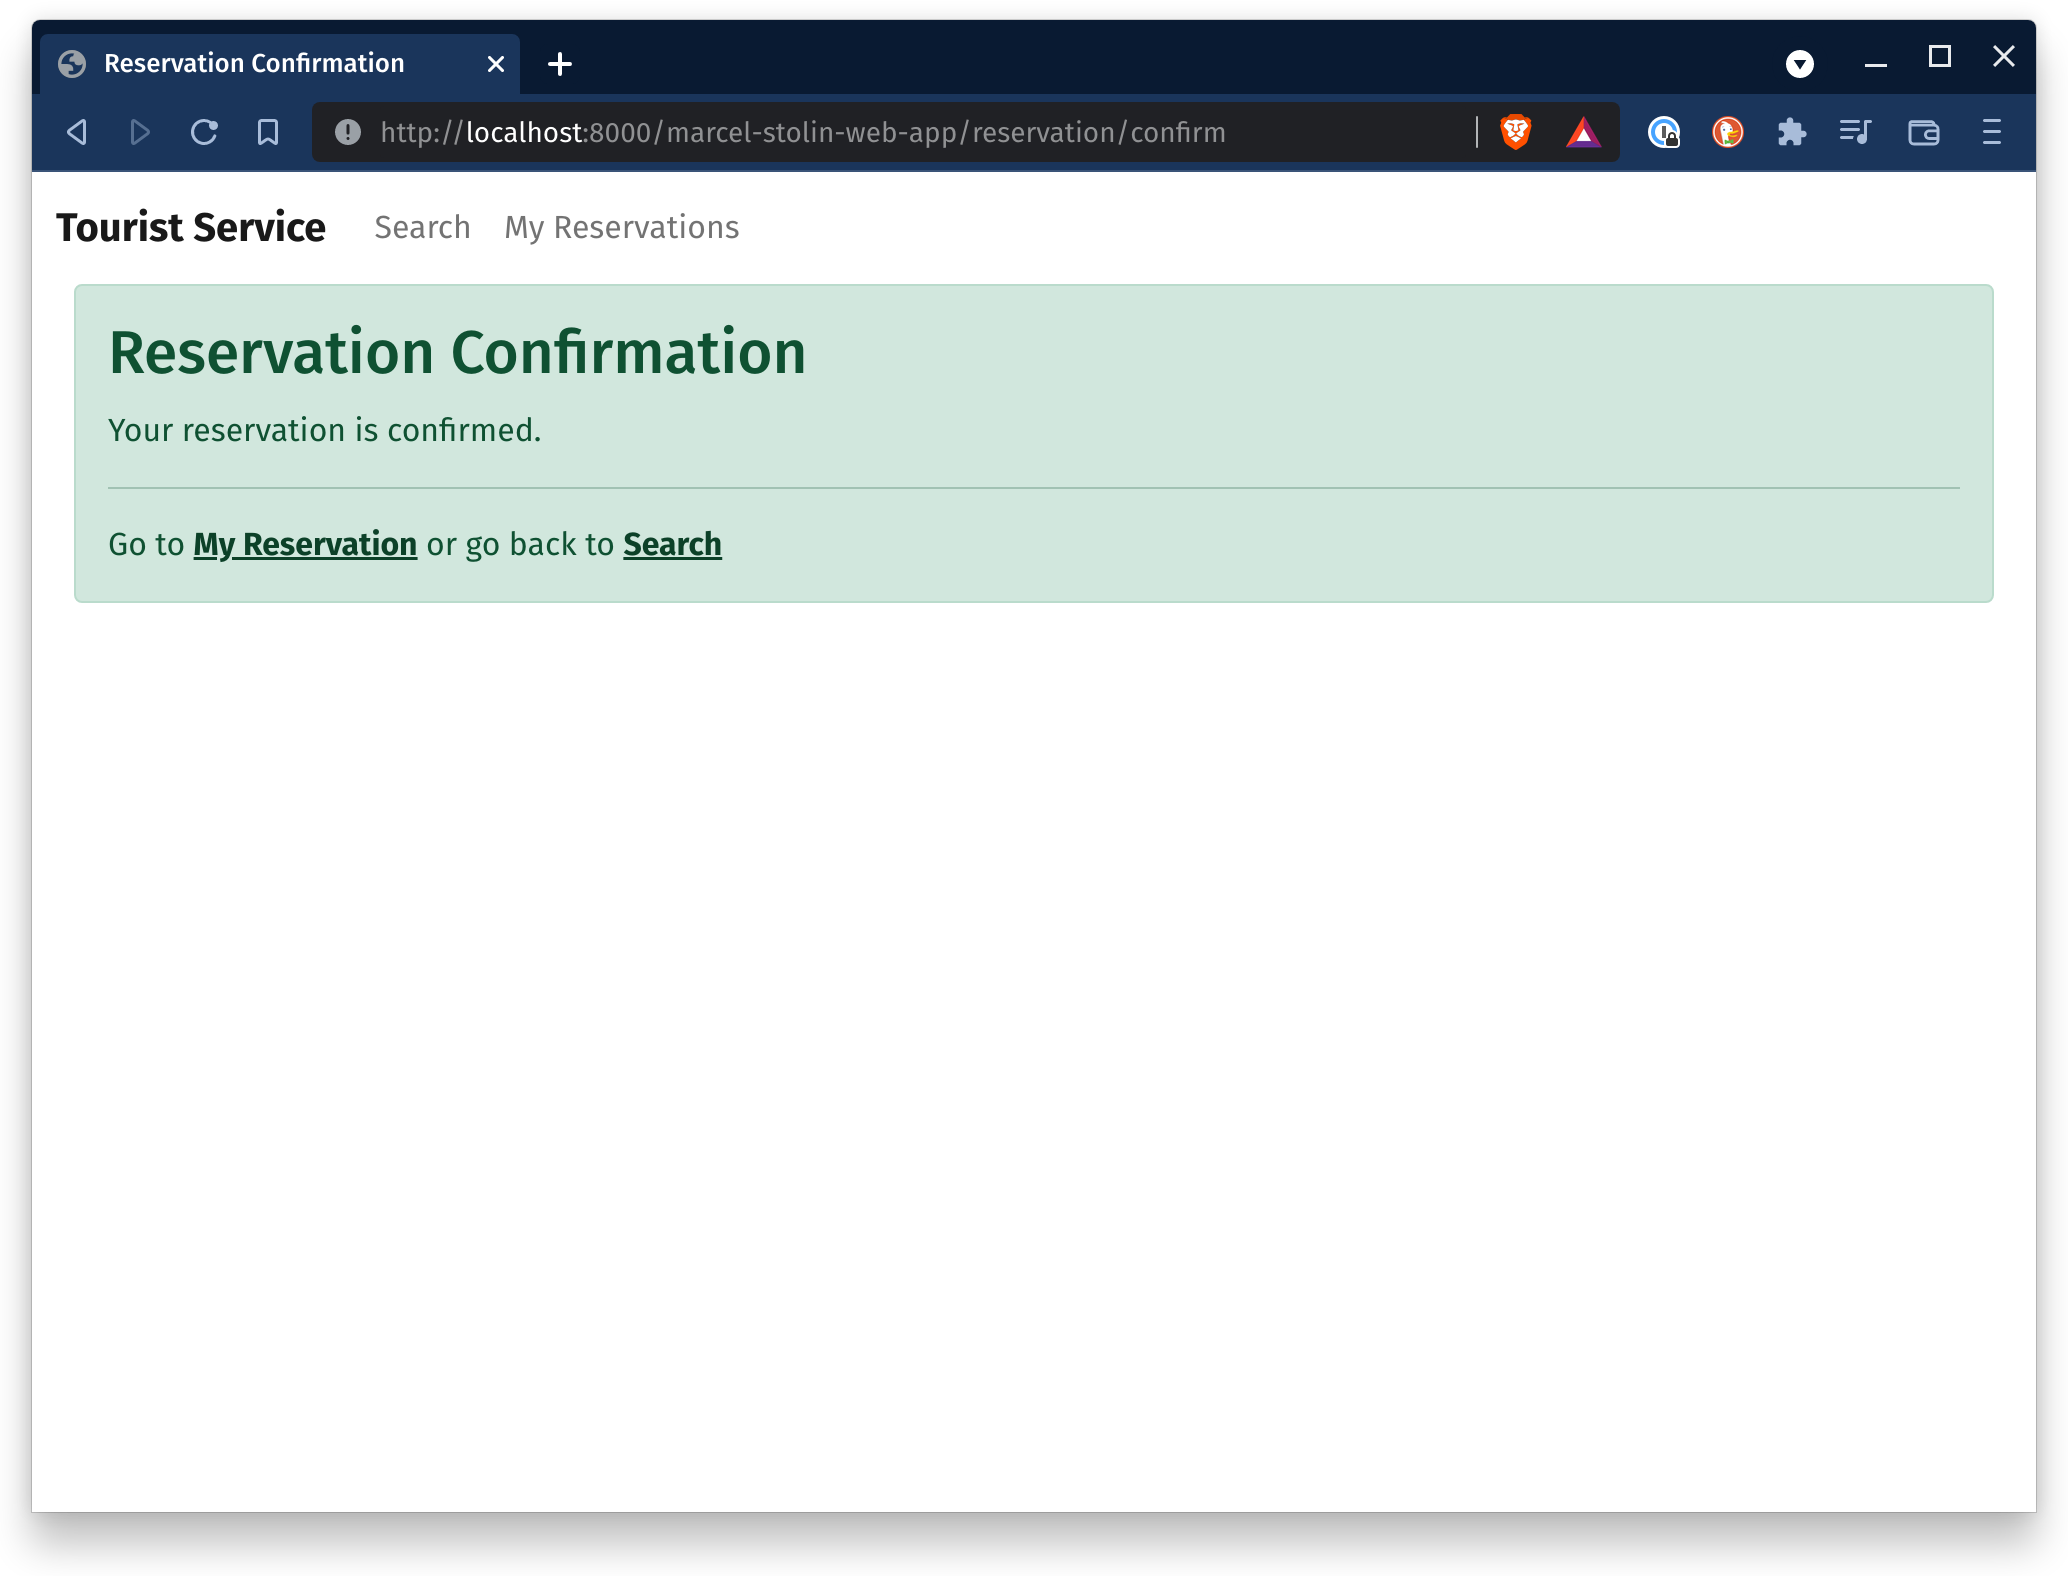
\includegraphics[scale=0.14]{images/02_design/web-app-reservation-confirm}
\caption{UI of the \textit{ReservationConfirmServlet}}
\label{fig:02_design_web_reservationconfirm_page}
\end{figure}

\subsubsection{ReservationListServlet}\label{sec:02_design_web_myreservations}
% What 
After a reservation has been confirmed, the user can look up all reservations at the \textit{ReservationListServlet}.
% How
There, the user has to provide the first name, and last name, same as given at the \textit{ReservationSummaryServlet} (introduced in \Sec{sec:02_design_web_reservationsummary}), shown in \Fig{fig:02_design_web_myreservations_page_1}. After submitting, the \textit{ReservationListServlet} sends a POST request to itself to present all reservations made by the given user, shown in \Fig{fig:02_design_web_myreservations_page_2}.

% Figure
\begin{figure}[h]
\centering
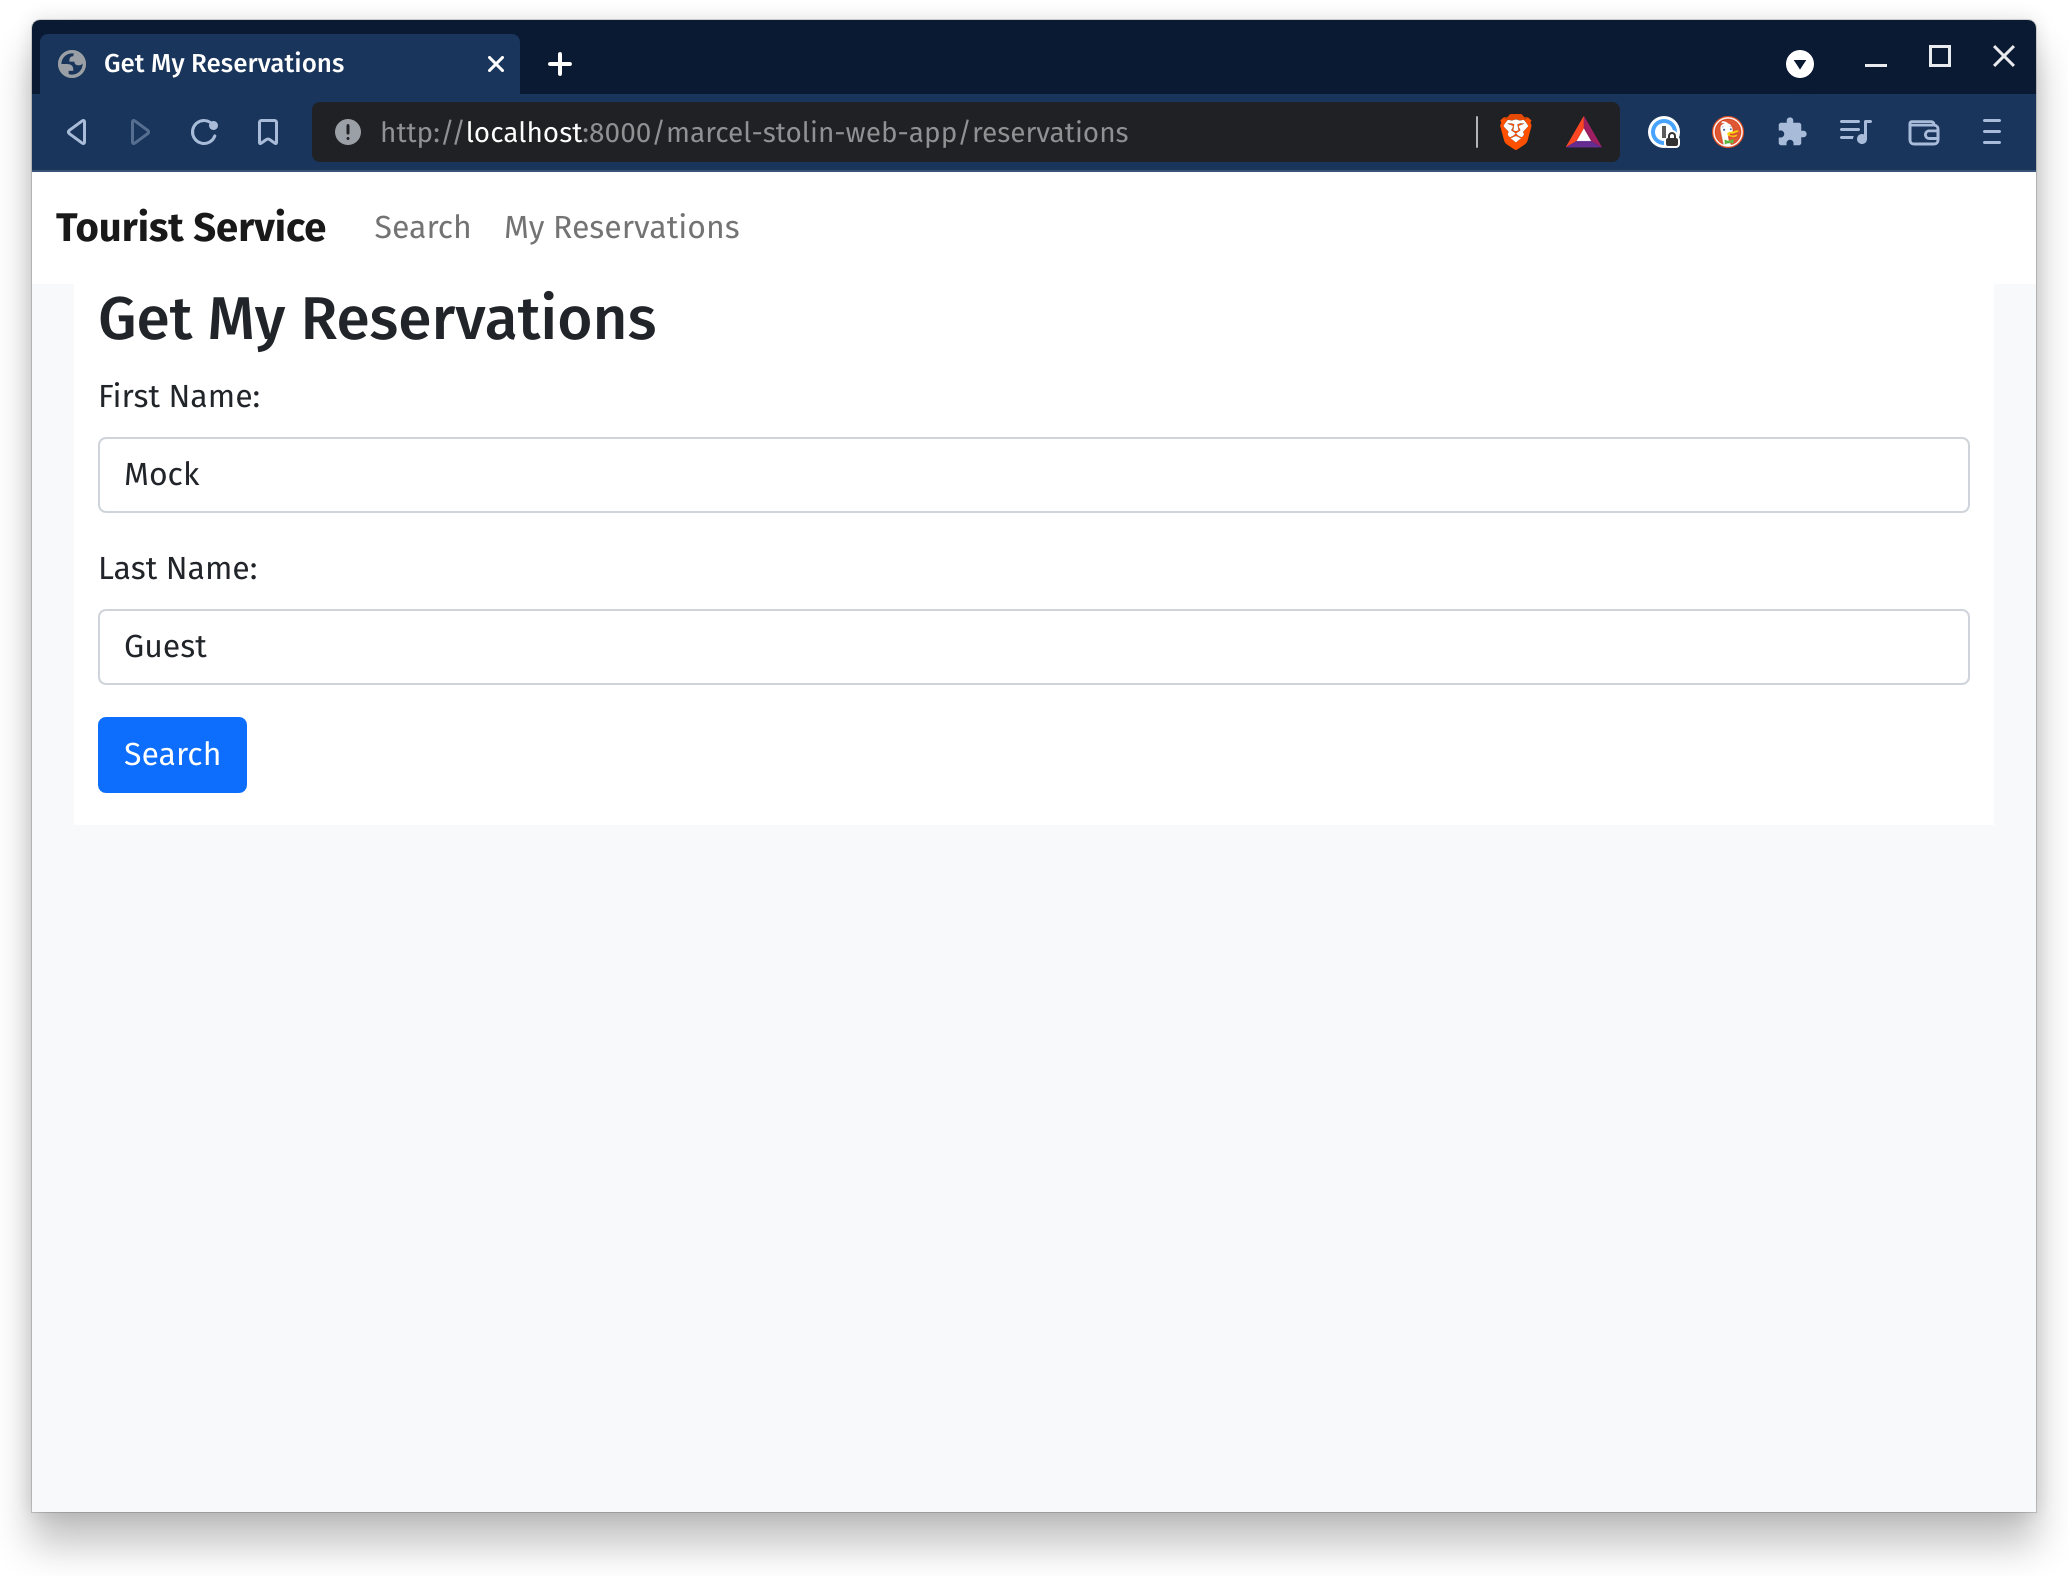
\includegraphics[scale=0.14]{images/02_design/web-app-my-reservations-1}
\caption{UI of the \textit{ReservationListServlet}}
\label{fig:02_design_web_myreservations_page_1}
\end{figure}

\newpage
% Figure
\begin{figure}[h]
\centering
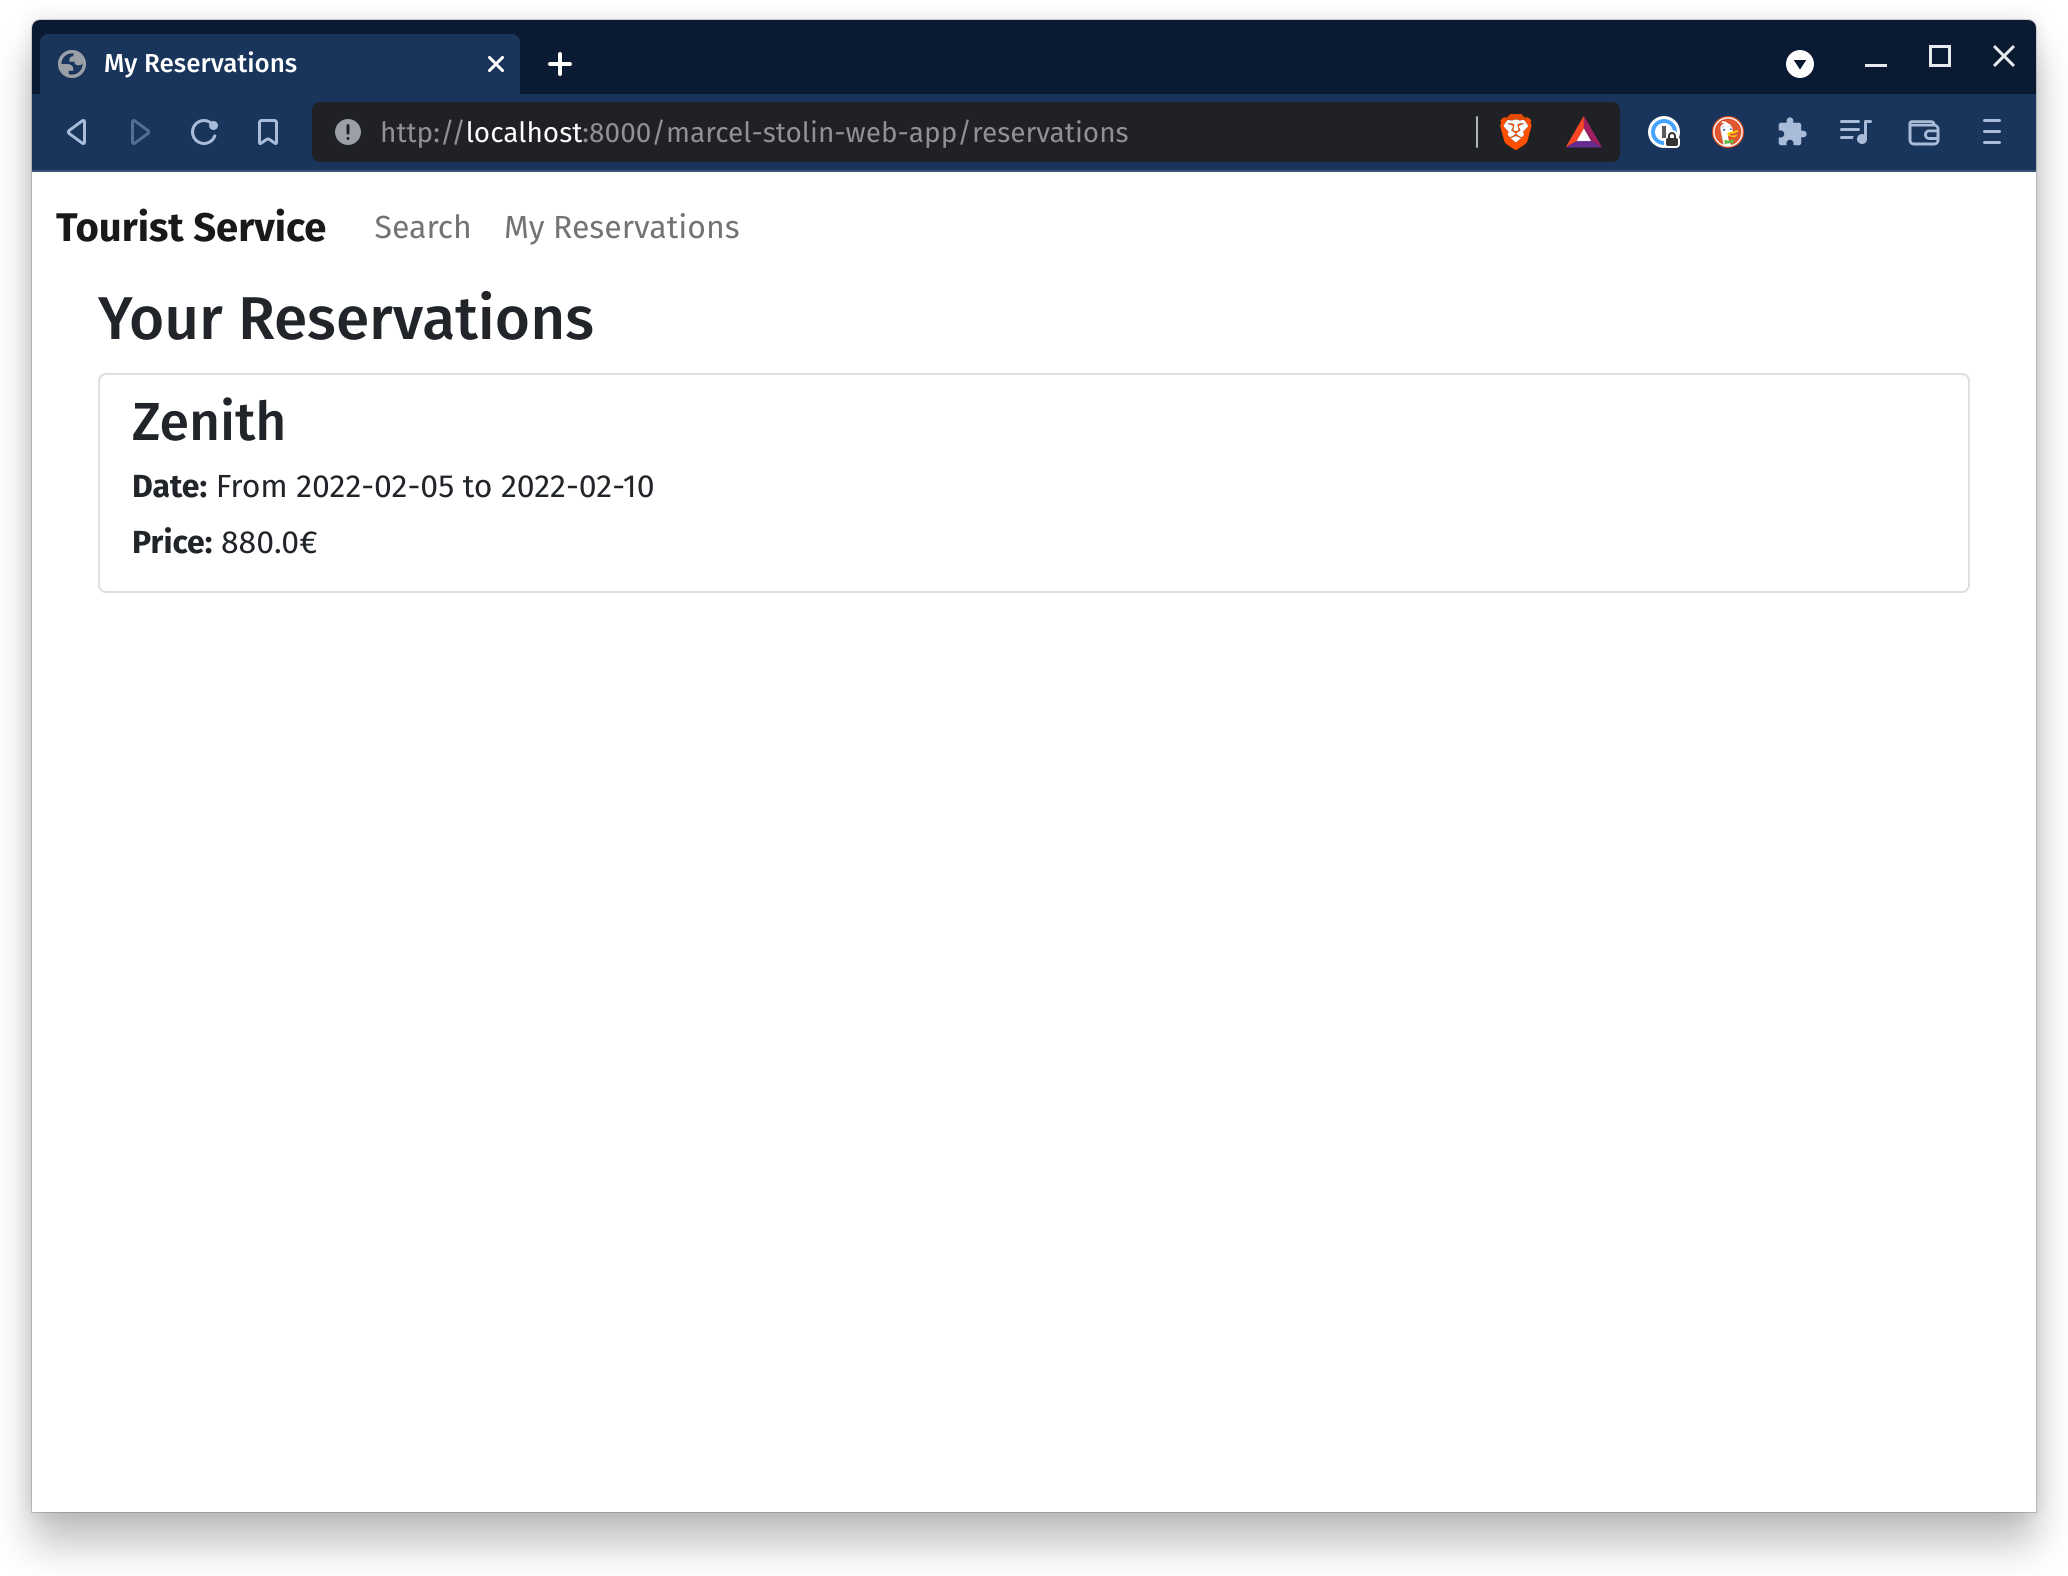
\includegraphics[scale=0.14]{images/02_design/web-app-my-reservations-2}
\caption{UI of the \textit{ReservationListServlet}}
\label{fig:02_design_web_myreservations_page_2}
\end{figure}
